\subsection*{Enana Blanca}

Una estrella nace de una nube molecular interestelar, una región de material ubicada en el espacio entre estrellas. Dependiendo de la masa inicial de el conjunto inicial de material es lo que determina las fases que la estrella pasa al envejecer. 

\begin{figure}
	\centering
	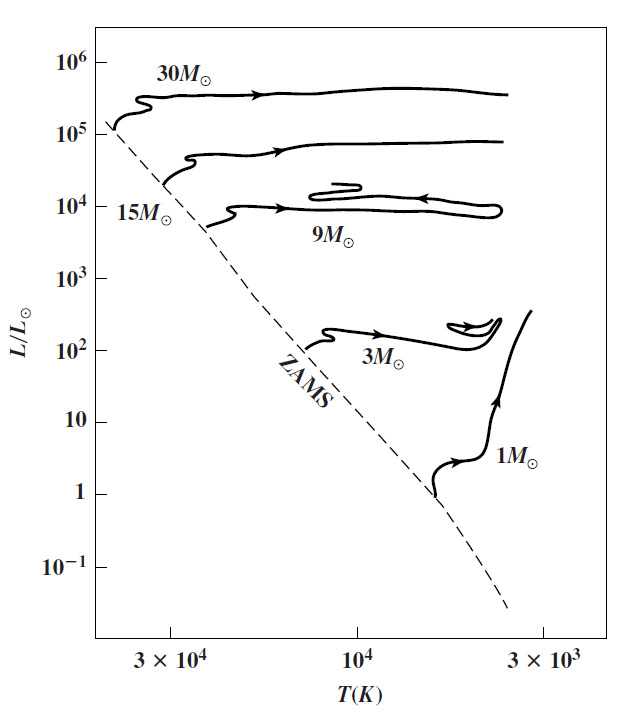
\includegraphics[scale=0.5]{Introduccion/Figures/Figura Evolucion_MS_Astronomy_Physical_Perspective.png}
	\caption{Evolución de estrellas de la secuencia principal basado en su masa inicial. Al consumir el hidrógeno en su núcleo por las reacciones nucleares que ocurren en esta misma región se comienza a desatar el equilibrio delicado que mantiene la forma de la estrella. Esta deformación provoca una oscilación en su tamaño, causado por las fluctuaciones del balance entre la presión radiativa generada por las reacciones nucleares en el núcleo contra la presión gravitacional.} \citet{astronomyPhysicalPerspective_stellarOldAgeChapter}
	\label{evolucionMSEstrella}
\end{figure}

Aquellas estrellas cuyas masas iniciales recae bajo 8.5-10.6 \(M_{\odot}\) terminan su vida como una estrella \textit{enana blanca.} (\citet*{whiteDwarfsReview}) 